\documentclass[12pt]{article}
% \usepackage[sc]{mathpazo} % Like Palatino with extensive math support
\usepackage[letterpaper, margin=1in]{geometry}
% \usepackage{mathptmx} % Like Times New Roman
\usepackage{newtxtext,newtxmath}
\usepackage{fullpage}
\usepackage[authoryear,sectionbib,sort]{natbib}

% The following works for line spacing for ESA journals
% (per http://esapubs.org/esapubs/latexTIPsESA.pdf):
\linespread{1.9}

\usepackage[utf8]{inputenc}
\usepackage{lineno}
\usepackage{titlesec}
\titleformat{\section}[block]{\Large\bfseries\filcenter}{\thesection}{1em}{}
\titleformat{\subsection}[block]{\Large\itshape\filcenter}{\thesubsection}{1em}{}
\titleformat{\subsubsection}[block]{\large\itshape}{\thesubsubsection}{1em}{}
\titleformat{\paragraph}[runin]{\itshape}{\theparagraph}{1em}{}[. ]\renewcommand{\refname}{Literature Cited}

% For Icelandic ð symbol:
\DeclareTextSymbolDefault{\dh}{T1}
% Increased spacing in math mode:
\medmuskip=8mu % by default it is equal to 4 mu
\thickmuskip=10mu % by default it is equal to 5 mu

% Figures
\usepackage{graphicx}
\graphicspath{ {./figures/} }
% Table
\usepackage{booktabs}


%%%%%%%%%%%%%%%%%%%%%
% Line numbering
%%%%%%%%%%%%%%%%%%%%%
%
% Please use line numbering with your initial submission and
% subsequent revisions. After acceptance, please turn line numbering
% off by adding percent signs to the lines %\usepackage{lineno} and
% to %\linenumbers{} and %\modulolinenumbers[3] below.
%
% To avoid line numbering being thrown off around math environments,
% the math environments have to be wrapped using
% \begin{linenomath*} and \end{linenomath*}
%
% (Thanks to Vlastimil Krivan for pointing this out to us!)

\title{Quantifying community responses to environmental variation from replicate
time series}



% This version of the LaTeX template was last updated on
% November 8, 2019.

%%%%%%%%%%%%%%%%%%%%%
% Authorship
%%%%%%%%%%%%%%%%%%%%%
% Please remove authorship information while your paper is under review,
% unless you wish to waive your anonymity under double-blind review. You
% will need to add this information back in to your final files after
% acceptance.

\author{
Joseph S. Phillips$^{1,2,3,\dagger}$ \\
Lucas A. Nell$^{1,4,\dagger}$ \\
Jamieson C. Botsch$^{1}$}



\usepackage{amsmath} % for split math environment


\date{}

% so that no commas are used in citations:
\bibpunct{(}{)}{,}{a}{}{,}


\begin{document}

\raggedright
\setlength\parindent{0.25in}

\maketitle


\noindent{} 1. Department of Integrative Biology, University of Wisconsin, Madison, Wisconsin 53706 USA

\noindent{} 2. Department of Aquaculture and Fish Biology, H\'{o}lar University, Skagafj\"{o}r{\dh}ur 551 Iceland

\noindent{} 3. E-mail: joseph@holar.is

\noindent{} 4. E-mail: lucas@lucasnell.com

\noindent{} $\dagger$ Both authors contributed equally.



\bigskip

Running head: {Community responses from time series}

% \textit{Manuscript elements}: %Figure~1, figure~2, table~1, online appendices~A and B (including $-- figure~A1 and figure~A2). Figure~2 is to print in color.

\linenumbers{}
% \modulolinenumbers[3]

\clearpage

% ---------------------------------------------------------------------------------------
% ---------------------------------------------------------------------------------------
% Abstract
% ---------------------------------------------------------------------------------------
% ---------------------------------------------------------------------------------------


\section*{Abstract}

Times-series data for ecological communities are increasingly available from
medium- and long-term studies designed to track responses to environmental change.
However, classical multivariate methods for analyzing community composition are
generally inappropriate for time series, as they do not account for temporal
autocorrelation in abundances of community members.
Furthermore, these traditional approaches often obscure the connections between
responses at the community level versus those for individual taxa, limiting
their capacity to infer the mechanisms of community change.
We show how linear mixed models with group-specific temporal autocorrelation can be
used to infer both taxon- and community-level responses to predictor variables from
replicated time series data.
Variation in taxon-specific responses to environmental predictors is modeled using
random effects.
These taxon-specific responses can be used to characterize variation in community
abundance and composition.
Furthermore, the degree of autocorrelation is estimated separately for each taxon as
this is likely to vary depending on the underlying population dynamics.
We illustrate the utility of the approach by analyzing the response of a predatory
arthropod community to spatiotemporal variation in allochthonous resources in a
tundra landscape.
Our results show how mixed models with temporal autocorrelation provide a unified
approach to characterizing taxon- and community-level responses to environmental
variation through time.


\bigskip

\textit{Keywords}: {allochthonous subsidies; autoregressive model; linear mixed model;
M\'{y}vatn; time-series analysis; tundra arthropods
}





% ---------------------------------------------------------------------------------------
% ---------------------------------------------------------------------------------------
% Introduction
% ---------------------------------------------------------------------------------------
% ---------------------------------------------------------------------------------------

\section*{Introduction}

A central goal of ecology is to understand how environmental variability affects
population and community dynamics.
Time series data of ecological communities collected from multiple sites across
large spatial scales are increasingly available from monitoring programs such as the
National Ecological Observatory Network \citep{Keller2008} and
long-term field experiments \citep[e.g.][]{Fraser2013, Cowles2018, Shi2015}.
Data of this sort provide great promise for answering long-standing questions about
how environmental factors drive community dynamics, but require the development of
appropriate analytical tools.

The response of ecological communities to environmental predictors is often analyzed
using ordination methods (e.g. NMDS, RDA), which map variation in abundance or
occurrence onto orthogonal axes that provide synoptic assessments of community
variation \citep{Mcgarigal2013}.
However, these methods are generally inappropriate for time-series data, as they
do not account for temporal autocorrelation in the abundance of members of the
community \citep{Ives2006}.
While some time-series methods have been developed for analyzing ecological communities,
these have generally focused on inferring interactions between species and therefore
require relatively long time series \citep{Ives1999, Hampton2013}.
In contrast, community time series are often relatively short but contain
replication through space or across experimental units, with the goal of
inferring the responses of communities to external drivers or experimental manipulations.

Here, we show how autoregressive mixed models (linear mixed models with temporal
autocorrelation structures) can be used to infer taxon- and community-level responses
to predictor variables from replicated time series data.
The approach is based on the method of \cite{Jackson2012}, who modeled variation in
taxon-specific responses to predictors as random effects.
We extend this approach for time series data by formulating models with separate
temporal autocorrelation structures for different taxonomic groups, accounting for
the fact that different taxa are likely to be characterized by different dynamics.
We then show how principle components analysis of predicted values from the model
can be used to visualize community variation along axes most associated with
environmental predictors, in a manner analogous to traditional ordination
\citep{Jackson2012}.
This approach has the advantage of making the connection between taxon- and
community-level variation explicit, while accounting for the autocorrelation
structure of time series data.

We illustrate the utility of this method by analyzing the responses of predatory
arthropods to spatiotemporal variation in allothchonous resources at Lake Mývatn
in northern Iceland \citep{Einarsson2004}.
Mývatn has large emergences of midges (Chironomidae) that subsidize the terrestrial
plant \citep{Gratton2008} and arthropod \citep{Dreyer2012, Sanchez2018} communities.
The midges have large interannual fluctuations \citep{Gardarsson2004} and decline
in deposition with distance from the lakeshore \citep{Dreyer2015}.
We apply autoregressive mixed models to assess the community response to the
highly variable midge subsidy, while also accounting for linear trends across
years and distance from the lake. This study shows how autoregressive mixed
models provide a unified approach for characterizing ecological responses to
environmental variation through time and space.







% ---------------------------------------------------------------------------------------
% ---------------------------------------------------------------------------------------
% Methods
% ---------------------------------------------------------------------------------------
% ---------------------------------------------------------------------------------------


\section*{Methods}

Lake M\'{y}vatn has a tundra-subarctic climate, with a surrounding landscape
dominated by heathland and grassland vegetation \citep{Einarsson2004}.
Arthropod samples were collected every 15$\pm$4d from five sites around the
shoreline of M\'{y}vatn from May to August in 2008 through 2019.
Each site included 3--4 plots at various distances
(5m, 50m, 150m, and 500m) along a transect perpendicular to the lakeshore.
Midge deposition was estimated at each site using aerial infall traps \citep{Dreyer2015},
and activity-density of ground-dwelling arthropods was sampled using pitfall traps
\citep{Southwood2009}.
Activity-density is a measurement of relative abundance, which represents a combination
of both population size and behavioral phenomena, both of which potentially respond
to the allochthonous inputs of resources \citep{Ostfeld2000}.
For this analysis, we used the cumulative annual catch of predatory and
detritivorous arthropods (Figure \ref{fig:obs-data}),
including ground beetles (Carabidae), rove beetles (Staphylinidae),
harvestmen (Opiliones), ground spiders (Gnaphosidae),
sheet-weaving spiders (Linyphiidae), and wolf spiders (Lycosidae).



We analyzed taxon-level variation across sites and years using an extension of
linear mixed models.
Our model included (1) fixed effects for predictor variables (number of years since initial
sampling year, distance from the lake, and midges);
(2) random intercepts grouped by taxon, site, and plot; and
(3) random slopes for the predictor variables grouped by taxon
(see appendix for full mathematical description).
The fixed effects give the average response across taxa to the predictor variables,
while the corresponding random effects give the deviation for each taxon from this
average response \citep{Jackson2012}.
The overall response of a given taxon is the sum of the corresponding fixed and
random components.
Quantifying responses for each taxon in a single model 
allows for "shrinkage" or “partial pooling” of the taxon-specific responses towards the mean response,
which reduces the noisiness of individual estimates and ameliorates concerns of multiple
comparisons \citep{Gelman2012} that have been raised for the examination of
responses for many taxa separately \citep{Mcgarigal2013}.
We log-transformed cumulative midges catch and distance and then z-scored (subtracted the mean 
and divided by the standard deviation) all predictors
(excluding the intercept).



To formulate the autoregressive component of the mixed model, we defined a vector $\mathbf{y}$
consisting of transformed counts for each taxon in each plot through time.
Because population processes are generally multiplicative, we log-transformed the counts,
adding one to all values to accommodate zeros.
We then z-scored the
transformed counts within each taxon to give the responses of different taxa on
comparable scales \citep{Jackson2012}.
The rows of $\mathbf{y}$ were grouped as individual time series
(i.e., taxon--plot combinations), with observations within each group ordered by time.
From this vector, we constructed a lagged vector $\mathbf{y\sp{\prime}}$,
where the first element for each time series was zero followed by the first through
penultimate observations for that time series \citep{Ives2006}.
This allowed us to specify an autoregressive model for the $i$th observation of
$\mathbf{y}$ as
%
\begin{equation} \label{eq:y-i}
\begin{split}
    y_i &= \mathbf{x}_i^\text{T} {\boldsymbol\beta}_i +
        \left( \phi_{\text{taxon}[i]} \right)^{\text{time}_i - \text{time}\sp{\prime}_i}
        y\sp{\prime}_i + \varepsilon_i \\
    \varepsilon_i &\sim \mathcal{N} \left(0, \; \sigma_{\text{residual}} \right)
    \text{,}
\end{split}
\end{equation}
%
\noindent where $\mathbf{x}_i^\text{T}$ is the transposed vector
of predictor values for the $i$th observation,
${\boldsymbol\beta}_i$ is a vector of coefficients 
modeled hierarchically according to the random effects structure described above,
$\phi_{\text{taxon}[i]}$ is the taxon-specific autoregressive (AR) parameter,
$\text{time}_i$ is the current time (in years),
$\text{time}\sp{\prime}_i$ is the lagged time (defined as for  $y\sp{\prime}$),
and $\varepsilon_i$  is the Gaussian residual
error with standard deviation $\sigma_{\text{residual}}$.
Because $y_i$ consists of log-transformed abundances, equation \ref{eq:y-i} is
essentially a log-linear model of population dynamics, with growth rate
$\mathbf{x}_i^\text{T} {\boldsymbol\beta}_i$ and
density-dependence $\phi_{\text{taxon}[i]}$
where values closer to zero indicate stronger regulation \citep{Ives2010, Ziebarth2010}.
Exponentiating the elapsed time with base $\phi_{\text{taxon}[i]}$ allows the model
to accommodate unequal time steps \citep{Zuur2009}.
The primary difference between the present approach and more traditional linear models
with AR structures \citep[e.g.][]{Zuur2009} is the estimation of separate values of the AR
parameter for different groups (i.e. taxa).
This is an important extension, as it allows different members of a community with
different levels of temporal autocorrelation (caused by differences in the underlying
dynamics) to be included in a single model.
We parameterized the model with the predictors giving the change in $y_i$,
rather than the mean of the stationary distribution as is often done
for autoregressive models \citep{Harvey1990, Ives2006},
because this reduced the correlation between the estimates of temporal trends and AR parameters.



Community analyses often utilize dimension reduction to characterize 
variation in community composition \citep{Mcgarigal2013}.
However, with our approach it is possible to infer variation in community composition 
directly from the variation in taxon-specific responses.
We illustrate this in two ways.
First, we compared the full model to a series of simplified models that either
(1) excluded the taxon-specific deviations from the mean
response (i.e. random effects) or (2) excluded the overall response across the
full community (i.e. fixed and random effects).
The former provided inference for variation in community composition per se,
while the latter provided inference for variation in both composition and overall abundance.
We made these comparisons using the Leave-one-out information criterion (LOOIC) \citep{Vehtari2017},
which is a Bayesian analogue to the Akaike information criterion (AIC) 
and can be similarly interpreted in units of deviance.
Second, we used principal components analysis on fitted values from the model
to generate orthogonal axes
characterizing the expected variation in the community due to the predictors
\citep[similar to][]{Jackson2012},
and we used ANOVA to partition variation in the fitted values 
into contributions from midges, time, and distance. 
We then projected the observed data onto these PC axes.
The total contribution of each predictor to the observed community variation
was calculated as the sum of the axis loadings weighted by 
the corresponding variance contributions.
These two approaches provided formal inference and visualization of community composition analogous 
to conventional ordination while appropriately accounting 
for temporal autocorrelation and maintaining an explicit link to taxon-specific responses. 



We fit the models with a Bayesian approach using Stan \citep{Carpenter2017},
via the \texttt{rstan} \citep{Stan2018} package in R.
We used 6 chains with 4000 iterations each (including 2000 iterations of "warm-up")
and assessed convergence based on effective sample size of the Markov chain, number of divergent
transitions, and potential scale reduction factor.
We used Gaussian priors with mean 0 and standard deviation 1 for the fixed effects,
Gamma priors with shape 1.5 and rate 3 for the standard deviations,
and Gaussian priors with mean 0 and standard deviation 0.5 for the AR parameter.
The latter was truncated with a lower bound of zero to avoid quasi-cyclic dynamics,
but did not have an explicit upper bound. 
Nonetheless, the estimated values of the AR parameters were less than one, indicating stationarity. 



% ---------------------------------------------------------------------------------------
% ---------------------------------------------------------------------------------------
% Results
% ---------------------------------------------------------------------------------------
% ---------------------------------------------------------------------------------------



\section*{Results}

There was a positive response of predator abundance to midge deposition,
as indicated by both the coefficient estimates (Figure \ref{fig:coefs}A,C)
and the modestly large improvement of the full model
relative to the reduced model (LOO deviance in Table \ref{tab:model-summary}).
The response to midges was somewhat variable across taxa,
as judged by the taxon-specific coefficients (Figure \ref{fig:coefs}A)
and the posterior distribution
for the random effect standard deviation (Figure \ref{fig:coefs}D).
However, this variation among taxa made a relatively small contribution
to the model fit (Table \ref{tab:model-summary}).
In contrast to the response to midges, there was large variation among taxa in
linear trends through time and distance from the lake (Figure \ref{fig:coefs}A,D),
and this taxon-specific variation dominated the contribution to the model fit
(Table \ref{tab:model-summary}).
Overall, the magnitudes of the taxon-specific responses to time and distance
were larger than the respones to midges.



The AR coefficients were generally similar across taxa and of modest magnitude,
indicating moderate levels of temporal autocorrelation across years
(Figure \ref{fig:coefs}B).
Ground spiders were an exception,
with an AR coefficient near zero indicating limited autocorrelation.
The relatively low autocorrelation is apparent from the time series,
where ground spiders appear more tightly constrained to their mean abundance
than was the case for other taxa (Figure \ref{fig:obs-data}A),
which results in less autocorrelated (i.e. ``faster'') fluctuations through time
\citep{Ziebarth2010}.



The first three PC axes contained all of the variation
due to linear effects of the three predictors and
collectively accounted for $\sim$68\% of the observed community variation
in abundance (Table \ref{tab:model-summary}).
Distance made the largest overall contribution,
followed by time and midges.
The effect of distance manifested almost exclusively through PC1,
while the effects of midges and time were both split between PC2 and PC3.
This indicates some degree of correspondence between linear responses of the community
to midges and time, as can be seen in taxon-specific coefficients
(Figure \ref{fig:coefs}A).
In contrast, the community response to distance
was largely uncorrelated with the responses to time and midges.



Although community-level results can be inferred from Figure \ref{fig:obs-data} and
Table \ref{tab:model-summary}, Figure \ref{fig:pca} illustrates how predictor effects
on the community can be visualized in a way similar to conventional ordination or
dimension-reduction methods widely used in community ecology.

The taxon-response vectors (Figure \ref{fig:pca}A)
provided information on the variation in overall abundance versus composition per se;
vectors of similar direction and magnitude
imply consistent responses across taxa (i.e. overall abundance),
while vectors of either different direction or magnitude imply variation in composition.
The direction of the taxon vectors was largely similar along PC2 (all positive
except for sheet weavers), reflecting the consistent overall
response of the community to midge deposition (Figure \ref{fig:pca}D).
In contrast, the direction and magnitude
of the taxon-vectors along PC1 was quite heterogeneous,
reflecting the fact that there was large variation in composition with
distance from the lake (Figure \ref{fig:pca}C).
Time had a similar effect on community composition per se, as can be seen when
projecting data onto PC2 and PC3 (Figure \ref{fig:pca-23}).
This contrast between effects on overall abundance versus composition
resulted directly from the relative magnitudes
of fixed versus taxon-specific random effects (Figure \ref{fig:coefs}),
illustrating the link between the two organizational scales.






% ---------------------------------------------------------------------------------------
% ---------------------------------------------------------------------------------------
% Discussion
% ---------------------------------------------------------------------------------------
% ---------------------------------------------------------------------------------------




\section*{Discussion}

Here, we show how linear mixed models with temporal autocorrelation can be used to
quantify community responses to environmental variation from replicated time series
observations.
Our approach extends the previous use of mixed models for estimating taxon- and
community-level responses to environmental variation through space
\citep{Jackson2012, Bartrons2015}, by incorporating temporal autocorrelation with
group-specific values for the autoregressive parameter.
This is an important extension, as taxa populations with different natural histories
likely have different degrees of autocorrelation in their population dynamics.
Furthermore, we show how predicted values from the model estimates can be combined
with principal components analysis \citep[following][]{Jackson2012} to visualize
community composition along axes of variation most strongly associated with
environmental variation.
This analysis makes explicit the connections between taxon- and community-level
variation and provides a conceptual link between the mixed model approach and
conventional ordination methods.


A central feature of our approach is its formulation in terms of taxon-specific
responses to environmental drivers, rather than aggregate measures of community
composition.
This stands in contrast to the previous approach of using some dimension-reduction
technique (e.g. PCA) to generate indices of community variation to use as
response variables in subsequent time-series analyses \citep{Simpson2009}.
In such analyses, the temporal autocorrelation structure of the aggregate measure
is a complex amalgamation of processes at lower levels of resolution.
This may be reasonable when the aggregate measure is of interest in and of itself,
for example when being used as a bioindicator of ecosystem status \citep{Bennion2015}.
However, community dynamics are manifestations of the dynamics of constituent populations.
Therefore, it will often be valuable to model the data in a fashion that preserves the
autocorrelation structure of those populations the community comprises.
The taxon-specific autoregressive parameter estimated by our approach has a
clear population-dynamic interpretation as the rate at which the population returns
to its central tendency, which in turn is closely tied to classical ecological
concepts of population regulation \citep{Nicholson1933, Ziebarth2010}.
This is a special case of a more general argument in favor of quantifying
taxon-specific variation rather than aggregate measures of composition,
following the motto that it is better to ‘analyze, then aggregate’ than it is to
‘aggregate, then analyze’ \citep{Clark2011}.



To illustrate its utility, we used our method to quantify the response of a predatory
arthropod community to spatiotemporal variation in allochthonous resources at
Lake M\'{y}vatn in northern Iceland.
We found a positive overall response of predator abundance to midge deposition,
which is consistent with previous studies at M\'{y}vatn
\citep{Hoekman2011, Hoekman2019, Dreyer2012, Sanchez2018} and
expected from studies of allochthonous subsidies in other systems
\citep{Murphy2012, Ostfeld2000, Yang2010}.
However, the variation among taxa in their responses to midges was fairly limited,
which means that variation in midge deposition was primarily associated with changes
in overall abundance in the community, rather than composition per se.
In contrast, trends in taxon abundance varied substantially across time and space,
which manifested as spatiotemporal variation in community composition.
Many of the factors determining the strength of pulsed allochthonous resources on
recipient communities \citep[e.g. landscape features;][]{Polis1997} also directly
affect the composition of the communities receiving those allochthonous inputs.
The ability of our modeling approach to partition variance between the spatiotemporal
patterns that affect both the community composition and the size of the allochthonous
inputs on the abundance of community members allowed for important insights into the
community dynamics of predators around Lake M\'{y}vatn.
Furthermore, this approach allowed for the utilization of long-term observational
data to gather the insights about the predatory arthropod community to natural
variation in allochthonous inputs, which represents an important contribution to the
allochthonous resource pulse literature \citep{Yang2008}.
Covariation between different drivers of ecological communities is common,
therefore this approach may have utility across many subdisciplines of community ecology.














% ---------------------------------------------------------------------------------------
% ---------------------------------------------------------------------------------------
% Acknowledgments
% ---------------------------------------------------------------------------------------
% ---------------------------------------------------------------------------------------
% You may wish to remove the Acknowledgments section while your paper
% is under review (unless you wish to waive your anonymity under
% double-blind review) if the Acknowledgments reveal your identity.
% If you remove this section, you will need to add it back in to your
% final files after acceptance.

% \section*{Acknowledgments}
%
% OEC would like to thank the world. GHC is much indebted to the solar system. AQE was supported by a generous grant from the Milky Way (MW/01010/987654).


% ---------------------------------------------------------------------------------------
% ---------------------------------------------------------------------------------------
% Appendices
% ---------------------------------------------------------------------------------------
% ---------------------------------------------------------------------------------------

% \newpage{}
%
% \input{app_A}


% ---------------------------------------------------------------------------------------
% ---------------------------------------------------------------------------------------
% Literature Cited
% ---------------------------------------------------------------------------------------
% ---------------------------------------------------------------------------------------



\bibliographystyle{ecology.bst}
\clearpage

\bibliography{refs.bib}


\clearpage

\begin{table}
\caption{\label{tab:model-summary}
Model inference.
LOO deviance was calculated from the posterior distribution of log-likelihoods
and compares the fit of the full model to a reduced model excluding either
deviations in taxon-specific responses from the mean response or
the overall response (including mean and taxon-specific components).
The scale of LOO deviance is comparable to $\Delta$AIC.
The variance partitioning was calculated using ANOVA,
with the sum-of-squares for each component scaled by the total sum-of-squares.
Parenthetical values show relative loadings for the PC axes.
The `Total' column is calculated as the sum across PC axes for each row,
with each axis weighted by the contribution of each predictor when relevant.}
\begin{tabular}{rrrrrrrr}
\toprule
 & \multicolumn{2}{c}{LOO deviance} & & \multicolumn{4}{c}{Variance partitioning} \\
 \cmidrule{2-3} \cmidrule{5-8}
 & \multicolumn{1}{c}{Taxon-variation} & \multicolumn{1}{c}{Overall} & &
    \multicolumn{1}{c}{PC1} & \multicolumn{1}{c}{PC2} & \multicolumn{1}{c}{PC3} &
    \multicolumn{1}{c}{Total} \\
& \multicolumn{1}{c}{(random)} & \multicolumn{1}{c}{(fixed + random)} & &
    \multicolumn{1}{c}{(0.34)} & \multicolumn{1}{c}{(0.17)} &
    \multicolumn{1}{c}{(0.17)} & \multicolumn{1}{c}{(0.68)} \\
\midrule
time & 37 & 34 &  & 0.00 & 0.28 & 0.84 & (0.19)\\
distance & 64 & 64 &  & 0.99 & 0.04 & 0.01 & (0.34)\\
midges & 4 & 15 &  & 0.01 & 0.67 & 0.15 & (0.14)\\
\bottomrule
\end{tabular}
\end{table}


\clearpage

\begin{figure}
\centering
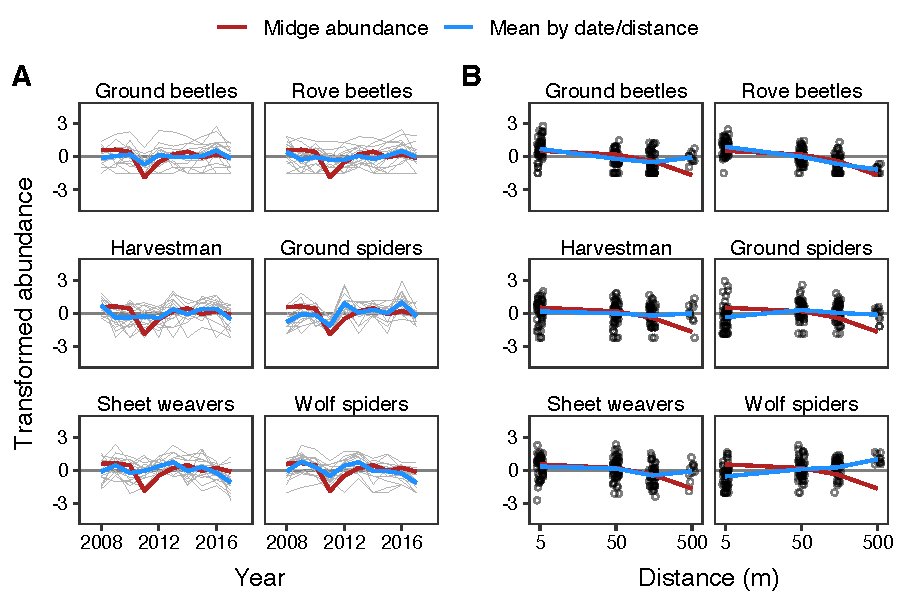
\includegraphics{fig1.pdf}
\caption{\label{fig:obs-data}
Community time series data for 6 predatory arthropod taxa at Lake M\'{y}vatn.
(A) Transformed abundance of arthropods through time.
Narrow gray lines are time series grouped by site and distance.
(B) Transformed abundance of arthropods versus distance from the lake.
Thick red lines are transformed midge abundances averaged by (A) year or (B) distance.
Thick blue lines are transformed abundances averaged by taxon and
(A) year or (B) distance.
Relative abundances were measured using activity-densities that were log-transformed,
then z-scored within each taxon.
}
\end{figure}




\clearpage

\begin{figure}
\centering
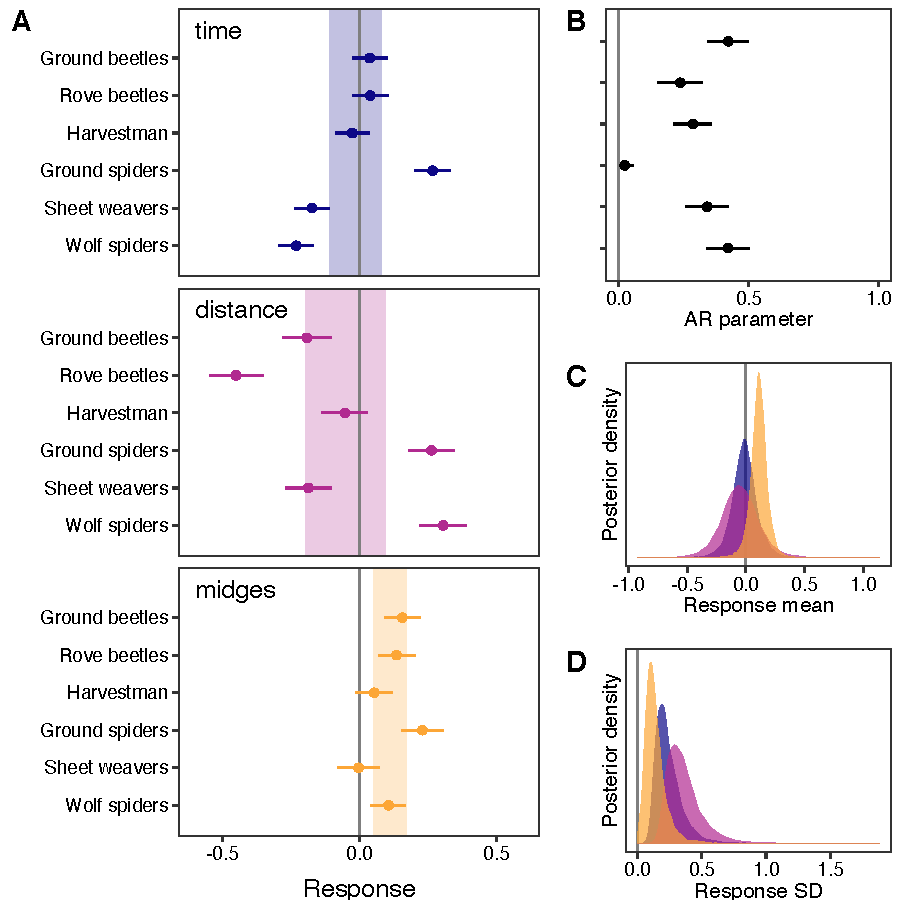
\includegraphics{fig2.pdf}
\caption{\label{fig:coefs}
Parameter estimates from the autoregressive mixed model, including
(A) taxon-specific responses to each predictor,
(B) autoregressive coefficients for each taxon, and
(C,D) posterior distributions for the fixed effects and random effect standard
deviations, respectively.
(A) The shaded regions correspond with the 68\% uncertainty interval
(analogous to the coverage of standard errors) for the mean response across taxa
(i.e. fixed effects shown in panel C).
(A,B) Points are posterior medians, and error bars are 68\% uncertainty intervals.
In all panels, gray vertical lines correspond to 0.
}
\end{figure}



\clearpage

\begin{figure}
\centering
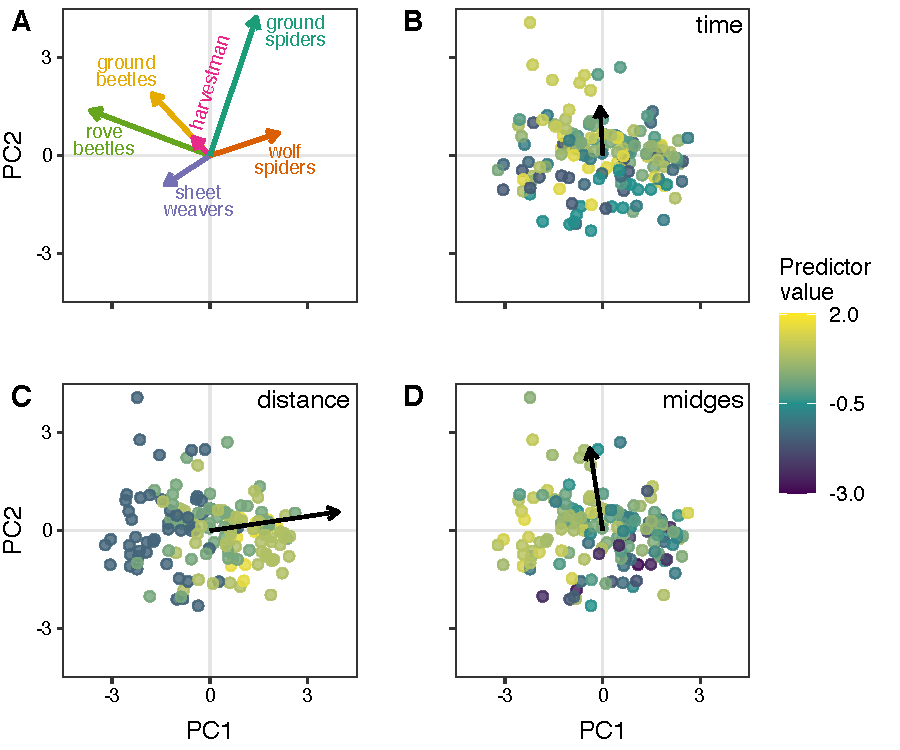
\includegraphics{fig3.pdf}
\caption{\label{fig:pca}
Principal components analysis (PCA) of community variation, showing
(A) taxon-response vectors and (B--D) model predictors projected onto the PC axes.
The PCA is based on the taxon-specific responses to time, distance, and midges,
as inferred from the model.
Therefore, the PC axes are aligned to maximize variation associated with responses
to the predictor variables, similar to ordination methods such as ``redundancy analysis.''
The observed data were then projected onto these axes so that variation accounted for
by the model could be visualized in the context of the data.
The taxon vector overlays in panel A are scaled relative to vectors in
B--D for clarity of visualization.
}
\end{figure}


% % Figure S1
% \caption{\label{fig:pca-23}
% Principal components analysis (PCA) of community variation, projected onto
% PC2 and PC3, showing (A) taxon-response vectors and
% (B--D) model predictors projected onto the PC axes.
% The PCA is based on the taxon-specific responses to time, distance, and midges,
% as inferred from the model.
% Therefore, the PC axes are aligned to maximize variation associated with responses
% to the predictor variables, similar to ordination methods such as ``redundancy analysis.''
% The observed data were then projected onto these axes so that variation accounted for
% by the model could be visualized in the context of the data.
% The taxon vector overlays in panel A are scaled relative to vectors in
% B--D for clarity of visualization.
% }
%
% % Figure S2
% \caption{\label{fig:pca-13}
% Principal components analysis (PCA) of community variation, projected onto
% PC1 and PC3, showing (A) taxon-response vectors and
% (B--D) model predictors projected onto the PC axes.
% The PCA is based on the taxon-specific responses to time, distance, and midges,
% as inferred from the model.
% Therefore, the PC axes are aligned to maximize variation associated with responses
% to the predictor variables, similar to ordination methods such as ``redundancy analysis.''
% The observed data were then projected onto these axes so that variation accounted for
% by the model could be visualized in the context of the data.
% The taxon vector overlays in panel A are scaled relative to vectors in
% B--D for clarity of visualization.
% }


\end{document}
